\documentclass[a4paper, 12pt]{article}

\usepackage[italian]{babel}
\usepackage{tikz}
\usepackage{xcolor}
\usepackage{graphicx}
\usepackage{hyperref}
\usepackage{imakeidx}
\usepackage{caption}
\usepackage{fancyhdr}
\usepackage{tabularx}


%--------------------VARIABILI--------------------
\def\logo{../Immagini/logo.jpeg}
\def\ultima-versione{v1.0}
\def\titolo{Verbale interno }
%------------------------------------------------

\usetikzlibrary{calc}
\definecolor{fp-blue}{HTML}{2885c8}
\definecolor{fp-red}{HTML}{ea5f64}
\makeindex[title=Indice]
\hypersetup{hidelinks}

\pagestyle{fancy}
\fancyhead[L]{}
\setlength{\headheight}{15pt}
\fancyhead[R]{\titolo - \ultima-versione}

\renewcommand{\familydefault}{\sfdefault}
\newcommand{\glossario}[1]{\fontfamily{lmr}\selectfont{\textit{#1\textsubscript{\small G}}}}

%--------------------INFORMAZIONI PRIMA PAGINA-------------------- 
\title{\Huge \textbf{\titolo}}
\author{\Large{Alt} \raisebox{0.3ex}{\normalsize  +} \Large{F4}}
\date{16 ottobre 2024}
%----------------------------------------------------------------

\begin{document}

\begin{titlepage}      
    \maketitle
    \thispagestyle{empty}  

    \begin{tikzpicture}[remember picture, overlay]
        \fill[fp-blue] 
        ($(current page.south west) + (0, 10)$) 
        -- ($(current page.center) + (0, -8)$)
        -- ($(current page.center) + (0, -15)$)
        -- (current page.south west);

        \fill[fp-red]
        ($(current page.south east) + (0, 10)$) 
        -- ($(current page.center) + (0, -8)$)
        -- ($(current page.center) + (0, -15)$)
        -- (current page.south east);

        \clip ($(current page.center) + (0, -8)$) circle (1cm) node 
        {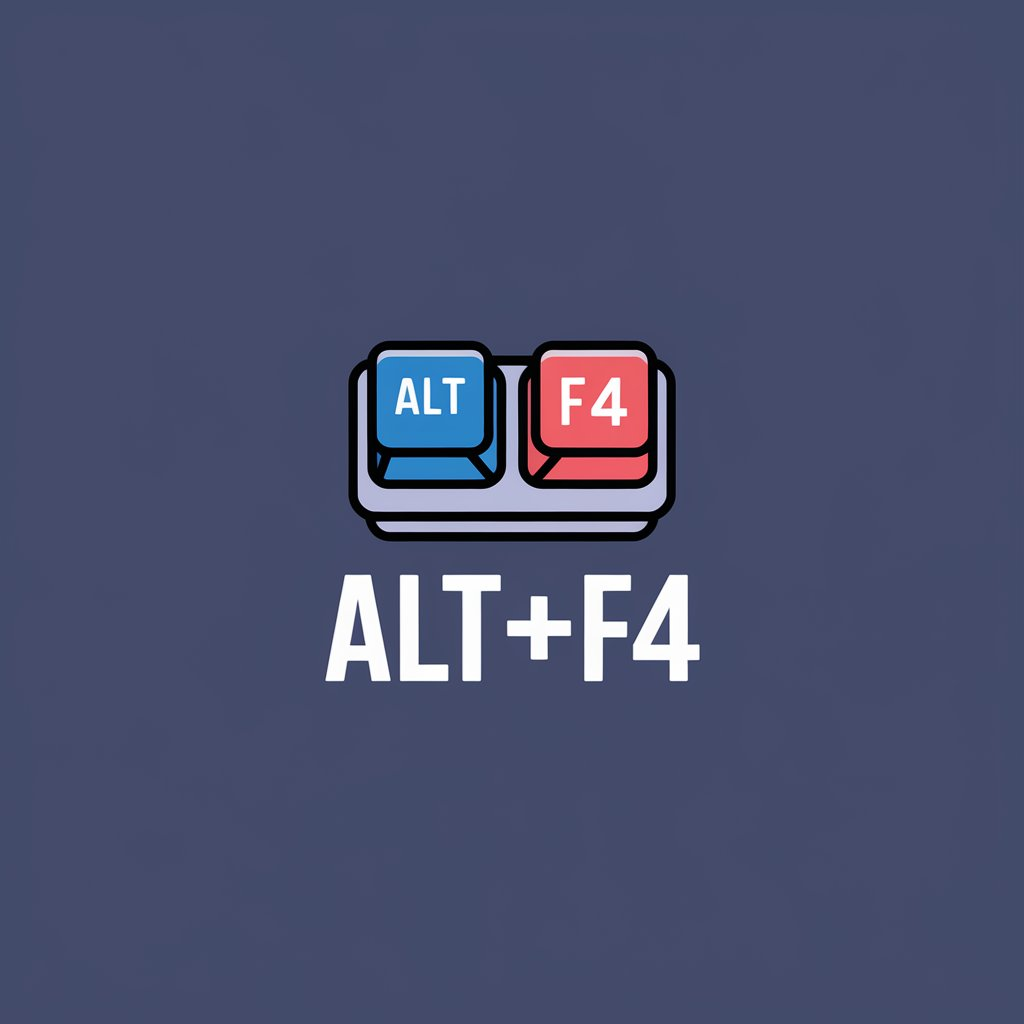
\includegraphics[width=.25\textwidth]{\logo}};
        
    \end{tikzpicture}    
\end{titlepage}

\tableofcontents

\newpage

\begin{table}[!h]
    \centering
    \caption*{\textbf{\Large Registro Modifiche}}
    {\renewcommand{\arraystretch}{2}
    \begin{tabularx}{\textwidth}{| X | X | X | X |}
        \hline
            \textbf{\large Versione} & 
            \textbf{\large Data} & 
            \textbf{\large Autore/i} & 
            \textbf{\large Descrizione} \\ 
        \hline \hline
        \ultima-versione & 
            30 ottobre 2024 & 
            Pedro Leoni & 
            Approvazione \\
        \hline 
            v0.2 & 
            30 ottobre 2024 & 
            Eghosa Matteo Igbinedion Osamwonyi & 
            Revisione \\
        \hline 
            v0.1 & 
            16 ottobre 2024 & 
            Francesco Savio & 
            Prima stesura del documento \\
        \hline
    \end{tabularx}}
\end{table}

\newpage
\section{Registro presenze}
\begin{itemize}
    \item[] \textbf{Data}: 16 ottobre 2024
    \item[] \textbf{Ora inizio}:  21:00
    \item[] \textbf{Ora fine}: 22:30
    \item[] \textbf{Piattaforma}: Discord	
\end{itemize}
\begin{table}[!h]
\centering
{\renewcommand{\arraystretch}{2}
\begin{tabularx}{\textwidth}{| X | X |}
    \hline
        \textbf{\large Componente} & 
        \textbf{\large Presenza} \\ 
    \hline 
    \hline
        Eghosa Matteo Igbinedion Osamwonyi&
        Presente \\
    \hline 
        Guirong Lan&
        Presente \\
    \hline 
        Enrico Bianchi&
        Presente \\
    \hline 
        Francesco Savio&
        Presente \\
    \hline 
        Marko Peric&
        Presente \\
    \hline 
        Pedro Leoni&
        Presente \\
    \hline 

\end{tabularx}}
\end{table}

\newpage

\section{Verbale}

Il primo incontro del gruppo avviene nella piattaforma discord ed inizia con una rapida
presentazione dei membri.
Dopo le presentazioni iniziali inizia a turno un'analisi sui capitolati e ogni 
componente esprime le preferenze per tre progetti in modo da stabilire quali sono i capitolati più interessanti per il gruppo e potersi candidare per essi.
Emerge un'interesse generale del gruppo abbastanza omogeneo e vengono prevalentemente discussi i capitolati C2,C5,C7 e C9. Dopo la scelta dei tre capitolati più stimolanti, in ordine 
di preferenza C9,C5 e C7 ci siamo proposti di contattarli nella settimana seguente.
Subito dopo c'è stato un brainstorming che ha avuto come scopo l’individuazione di un nome che possa piacere a tutti i membri.
Dopo aver selezionato varie alternative senza arrivare ad un nome definitivo condiviso da tutti è stato scelto di affidare al caso la scelta del nome, Guirong Lan ha impostando uno strawpoll con i nomi più belli. Il nome scelto è "Alt+F4".
Successivamente il componente Eghosa Matteo Igbinedion Osamwonyi si è offerto per la realizzazione di varie grafiche per il logo tramite AI che verranno votate successivamente al fine di scegliere quello preferito dal gruppo.
Successivamente Francesco Savio si è offerto di creare la mail del gruppo utilizzando come provider gmail.
Gli ultimi minuti sono stati dedicati ad accennare delle tecnologie del way of working del gruppo che verranno usate in questa fase iniziale, in particolare Pedro Leoni ha consigliato di utilizzare LaTeX per la preparazione dei documenti, e successivamente si è concordato di utilizzare GitHub per la creazione di un repository di gruppo.


\section{To Do}
\begin{itemize}
    \item Contattare tramite mail le aziende dei capitolati C9,C5 e C7.
    \item Scegliere il logo tra quelli proposti da Matteo.
    \item Creazione del repository GitHub.
    \item Creazione di un template latex e studio di latex per i membri del gruppo che non lo conoscono.
\end{itemize}

\end{document}